\subsection{Uebersicht}\label{uebersicht}
Die Komponente “App und Datenbankhandling” besteht zum wesentlich aus diese drei Unterkomponenten.
\begin{figure}[htb]
 \centering
 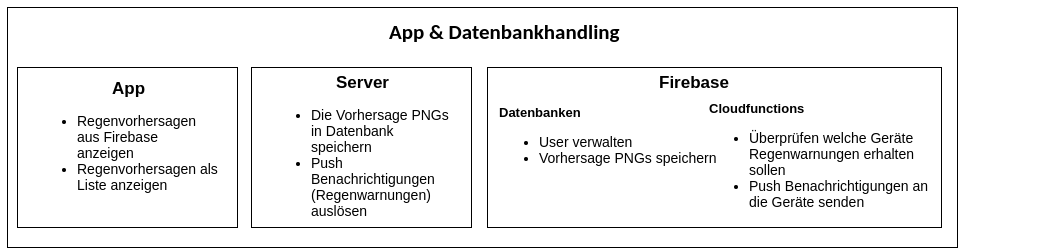
\includegraphics[width=0.6\textwidth,angle=0]{abb/app_datenbank_komponente_uebersicht}
 \caption[Beschreibung]{Übersicht über die im folgenden Kapitel betrachtete Komponente App und Datenbankhandling}
\label{fig:Beschreibung}
\end{figure}

Die App dient im Wesentlichen zur Visualisierung der Daten und macht somit die Regenvorhersagen für den Endnutzer brauchbar. Auf dem Server werden die Vorhersagen berechnet und, in dem für dieses Kapitel relevanten Teil, für die App zur Verfügung gestellt. Die Cloudfunktion, welche in der Firebase gespeichert ist, ist für das senden der Push Benachrichtigungen an das Gerät verantwortlich. Das senden der Push Benachrichtigungen wird jedoch vom Server getriggert.  